\documentclass[12pt]{article}
\usepackage{geometry} % see geometry.pdf on how to lay out the page. There's lots.
\geometry{a4paper} % or letter or a5paper or ... etc
\usepackage{graphicx}

% \geometry{landscape} % rotated page geometry

% See the ``Article customise'' template for come common customisations

\title{GoLisp}
\author{Dave Astels}

\begin{document}

\maketitle

\section{Overview}

GoLisp is a simple Lisp implimented in Go for integrating into a Go
application to provide runtime extension and scripting. The core of a
basic Lisp in provided, but with limited special forms and primitive
functions. More of these will be added as required. 

\section{Data types}

\begin{description}

\item[Cons Cells] are the central data type in classic Lisp used for
  both as dotted pairs \verb|(a .  b)| and general lists \verb|(a b)|.
  A cons cell is made up of two pointers, the \verb|car| and
  \verb|cdr|, as shown in Figure~\ref{fig:conscell}.

\begin{figure}[htbp] %  figure placement: here, top, bottom, or page
   \centering
   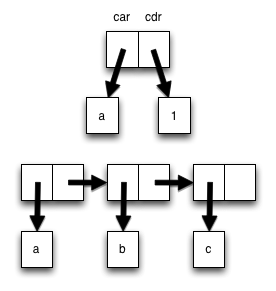
\includegraphics[width=5in]{conscell.png} 
\caption{Cons Cell.}
\label{fig:conscell}
\end{figure}

\item[Symbols] are simple identifiers, e.g. \verb|function-name|.
Symbols follow the follow simple rules: 

\begin{itemize}
\item starts with a letter, and
\item contains alphanumeric, \verb|-|, \verb|?|, and \verb|!|.
\end{itemize}

Typically, \verb|-| is used to seperate words in a symbol, \verb|?| is
used at the end of the name of a predicate function, and \verb|!| is
used at the end of the name of a fucntion that changes some state as a
side effect (\verb|set!| is a canonical example).

Some builtin function names violate these rules (e.g. arithmetic and
relative functions). You can't create symbols like this without
adding support for them to the parser.

\item[Strings] are any sequence of characters other than \verb|"|
enclosed by a pair of \verb|"|, e.g. \verb|"string"|.

\item[Numbers] are integers internally represented as \verb|int| so
  their size reflects \verb|int| on the build of Go being used. E.g.
  \verb|5|, \verb|9845376|. 

\item[Booleans] represent true and false. \verb|nil|, \verb|()|, and
false are all logically false, everything else is logically true.
Boolean literals are \verb|#t| and \verb|#f| for true and false,
respectively. 

\item[Functions] are user defined procedures. They are covered in
detail later.

\item[Objects] allow you to encapsulate a Go object (struct) in a Lisp
  data object. There is no way to do this from Lisp itself, but is
  useful when writing primitive functions (see below). 

\item[Primitives] are just as they are in Lisp or Smalltalk: functions
  written in Go and exposed as functions in Lisp. The combination of
  primitives and objects allow you to integrate with the underlying Go
  program. 

\end{description}

\section{Builtin functions}

\noindent{\bf\verb|(+ <number>...)|}

Adds a series of numbers, e.g.

\begin{verbatim}
    (+ 4) ==> 4
    (+ 4 2) ==> 6
    (+ 4 2 7) ==> 13
\end{verbatim}

\noindent{\bf\verb|(- <number>...)|}

Sequentially subtracts a sequence of numbers. With a single argument
is a special case that negates the argument. E.g. 

\begin{verbatim}
    (- 4) ==> -4
    (- 10 3) ==> 7
    (- 10 3 4) ==> 3
    (- 10 3 4 5) ==> -2
\end{verbatim}

\noindent{\bf\verb|(* <number>...)|}

Multiplies a series of numbers, e.g.

\begin{verbatim}
    (+ 4) ==> 4
    (+ 4 2) ==> 6
    (+ 4 2 7) ==> 13
\end{verbatim}

\noindent{\bf\verb|(/ <number>...)|}

Sequentially divides a sequence of numbers. E.g.

\begin{verbatim}
    (/ 30 2) ==> 15
    (/ 30 2 3 ) ==> 5
\end{verbatim}

\noindent{\bf\verb|(% <number> <number>)|}

Returns the remainder of dividion. E.g.

\begin{verbatim}
    (% 4 2) ==> 0
    (% 4 3) ==> 1 
\end{verbatim}

\noindent{\bf\verb|(< <number> <number>)|}

Returns whether the first argument is less than the second argument.

\begin{verbatim}
    (< 1 2) ==> #t
    (< 2 1) ==> #f
    (< 2 2) ==> #f
\end{verbatim}

\noindent{\bf\verb|(> <number> <number>)|}

Returns whether the first argument is greater than the second argument.

\begin{verbatim}
    (> 1 2) ==> #f
    (> 2 1) ==> #t
    (> 2 2) ==> #f
\end{verbatim}

\noindent{\bf\verb|(== <number> <number>)|}

Returns whether the first argument is equal to the second argument.

\begin{verbatim}
    (== 1 2) ==> #f
    (== 1 1) ==> #t
\end{verbatim}

\noindent{\bf\verb|(!= <number> <number>)|}

Returns whether the first argument is not equal to the second argument.

\begin{verbatim}
    (!= 1 2) ==> #t
    (!= 1 1) ==> #f
\end{verbatim}

\noindent{\bf\verb|(<= <number> <number>)|}

Returns whether the first argument is less than or equal to the second
argument. 

\begin{verbatim}
    (<= 1 2) ==> #t
    (<= 2 1) ==> #f
    (<= 2 2) ==> #t
\end{verbatim}

\noindent{\bf\verb|(>= <number> <number>)|}

Returns whether the first argument is greater than or equal to the
second argument. 

\begin{verbatim}
    (>= 1 2) ==> #f
    (>= 2 1) ==> #t
    (>= 2 2) ==> #t
\end{verbatim}

\noindent{\bf\verb|(! <arg>)|}

Returns whether the boolean negation of the argument.

\begin{verbatim}
    (! #t) ==> #f
    (! #f) ==> #t
\end{verbatim}

\section{Special forms}

\noindent{\bf\verb|(if <condition> <true clause>)|}

If the condition evaluates to logically true, the true clause is
evaluated and the result is the result of the if form, otherwise nil
is the result of the if form. 

\begin{verbatim}
    (if (< 1 2) 
        "less") ==> "less"
    (if (< 2 2) 
        "less") ==> nil
\end{verbatim}

\noindent{\bf\verb|(if <condition> <true clause> <else clause>)|}

If the condition evaluates to logically true, the true clause is
evaluated and the result is the result of the if form, otherwise the
else clause is evaluated and is the result of the if form. 

\begin{verbatim}
    (if (< 1 2) 
        "less" 
        "not less") ==> "less"
    (if (< 2 2) 
        "less" 
        "not less") ==> "not less"
\end{verbatim}

\noindent{\bf\verb|(lambda (<param>...) <expr>...)|}

Creates an anonymous function. This can then be used in a function call.

\begin{verbatim}
    ((lamdba (x) 
       (+ x x)) 
     5) ==> 10
\end{verbatim}

\noindent{\bf\verb|(define <symbol> <value>)|}

Evaluates the value expression and binds it to the symbol, returning
the value. 

\begin{verbatim}
    (define x (+ 2 3)) ==> 5
    x ==> 5
\end{verbatim}

Functions can be named (i.e. bound to a symbol) and later referred to
by using define:

\begin{verbatim}
  (define foo (lamdba (x) 
                (+ x x)))
  (foo 5) ==> 10  
\end{verbatim}


\noindent{\bf\verb|(define (<symbol> <param>...) <body>)|}

A syntacticly cleaner way to name a function:

\verb|<symbol>| specifies the name (how you reference the function)

\verb|<param>...| parameters of the function, these are bound to the
respective arguments when the function is called. 

\verb|<body>| the sequence of expressions that are evaluated in order
when the function is called. The final evaluation result becomes the
value of evaluation of the function. 

\begin{verbatim}
    (define (double x)
       (+ x x))
    (double 5) ==> 10
\end{verbatim}

\noindent{\bf\verb|(quote <expr>)|}

Surpresses evaluation of the expression.

\begin{verbatim}
     (quote (+ 1 2)) ==> (+ 1 2)
\end{verbatim}

There is a shortcut for quote that uses the single quote:

\begin{verbatim}
    '(+ 1 2) ==> (+ 1 2)
\end{verbatim}

\noindent{\bf\verb|(map <function> <list>)|}

Applies \verb|function| (which has to be of a single argument) to each
element in \verb|list| in order, returning the list of the results. 

\begin{verbatim}
    (map - '(1 2 3 4)')) ==> (-1 -2 -3 -4)

    (map (lambda (x)
                 (* x x))
         '(1 2 3 4)') ==> (1 4 9 16)
\end{verbatim}

\noindent{\bf\verb|(being <sexpr>...)|}

Evaluates the each \verb|sexpr| in order, returning the result of the
last one evaluated. Used in a context that allows a single
\verb|sexpr| but you need multiple. E.g.

\begin{verbatim}
  (if (predicate)
      (begin
        (do-something)
        (do-something-else)))
\end{verbatim}

\noindent{\bf\verb|(let ((<name> <value>)...) <sexpr>...)|}

Create a local scope and bindings for evaluating a body of code. The
first argument is a list of bindings. Each binding is a raw symbol
(doesn't get evaluated) that is the name to be bound, and a value
(which is evaluated). These bindings are added to a scope that is
local to the let. The body is evaluated in this local scope. The value
of the \verb|let| is the last evaluation result. E.g.

\begin{verbatim}
  (let ((x 1)
        (y 2))
       (+ x y)) ==> 3
\end{verbatim}

Bindings cascade. I.e. each binding's value is evaluated in the
context of the local scope. E.g.

\begin{verbatim}
  (let ((x 1)
        (y (+ x 2)))
       (+ x y)) ==> 4
\end{verbatim}

As mentioned above, \verb|let| takes a sequence of sexprs as it's
body. In effect the body of the \verb|let| is an implicit
\verb|begin|.

\begin{verbatim}
  (let ((x 1)
        (y (+ x 2)))
       (do-something)
       (+ x y)) ==> 4
\end{verbatim}

\section{Defining primitives}

The Go function \verb|MakePrimitiveFunction| allows you to create
primitive functions. This takes three arguments:

\begin{enumerate}
\item The function name. This is the name of a symbol which will be
  used to reference the function. 
\item The number of expected arguments. Using a -1 for this denotes
  any number of arguments. In the function definition you can enforce
  further constraints on argument counts and types. 
\item The Go function which impliments the primitive. This function
  {\bf must} have the signature
  \verb|func <Name>(args *Data) (result *Data, err error)| 
\end{enumerate}

\noindent An example:

\begin{verbatim}
    MakePrimitiveFunction("!", 1, BooleanNot)

    func BooleanNot(args *Data) (result *Data, err error) {
        if Length(args) != 1 {
            err = errors.New(fmt.Sprintf("! requires 1 argument. Received %d.", Length(args)))
            return
        }

        arg, err := Eval(Car(args))
        if err != nil {
            return
        }

        val := BooleanValue(arg)
        return BooleanWithValue(!val), nil
     }
\end{verbatim}

\subsection{Data}

The core lisp data element is the data type which logically
contains a type tag and a value. The type tags are defined by the
constants: 

\begin{description}
\item[ConsCellType] 
\item[NumberType]
\item[BooleanType]
\item[StringType]
\item[SymbolType]
\item[FunctionType]
\item[PrimitiveType]
\item[ObjectType]
\end{description}

\noindent The types are described earlier. If you need to check the
type of a piece of data you can fetch it's type using the
\verb|TypeOf(*Data) int| fuction and then compare it to a type tag
constant. Additionally there are predicate functions for the most
common types: 

\begin{description}
\item [{\tt StringP(*Data) bool}] returns whether the data is a string
\item [{\tt SymbolP(*Data) bool}] returns whether the data is a symbol
\item [{\tt NumberP(*Data) bool}] returns whether the data is a number
\item [{\tt PairP(*Data) bool}] returns whether the data is a cons cenn
  (aka pair)
\item [{\tt ObjectP(*Data) bool}] returns whether the data is an
  encapsulated Go object 
\item [{\tt FunctionP(*Data) bool}] returns whether the data is either
  a user defined or primitive function
\end{description}

\noindent Two other very handy functions are:

\begin{description}
\item [{\tt NilP(*Data) bool}] returns whether the data is nil
\item [{\tt NotNilP(*Data) bool}] returns whether the data is non-nil
\end{description}

\section{Creating and accessing data}

There are various convience functions that you can use to create data:

\begin{description}
\item [{\tt Cons(car *Data, cdr *Data) *Data}] creates a cons cell
  with the provided values for it's \verb|car| and \verb|cdr|.
\item [{\tt NumberWithValue(n int) *Data}] creates a number (integer)
  with the provided value
\item [{\tt BooleanWithValue(b bool) *Data}] creates a boolean with
  the provided value
\item [{\tt StringWithValue(s string) *Data}] creates a string with
  the provided value
\item [{\tt SymbolWithName(s string) *Data}] creates a symbol with the
  provided name
\item [{\tt ObjectWithTypeAndValue(thpeName string, o unsafe.Pointer) *Data}]
  creates an encapsulated Go object with the given type tag\footnote{a
    string eqivalent to the Go type of the value} and value 
\end{description}

\noindent Similarly there are functions for extracting information
from data elements: 

\begin{description}
\item [{\tt IntValue(*Data) int}] extracts the primitive integer value
\item [{\tt StringValue(*Data) string}] extracts the primitive
  string value
\item [{\tt BooleanValue(*Data) bool}] extracts the primitive
  boolean value
\item [{\tt TypeOfObject(*Data) string}] extracts the type tag of the
    encapsulated Go object
\item [{\tt ObjectValue(*Data) unsafe.Pointer}] extracts the
  primitive object value
\item [{\tt String(*Data) string}] returns a human readable string
  representation of the data 
\item [{\tt Length(*Data) int}] returns the length of a piece of Lisp 
  data. This will be 0 in all cases except lists, when it will be the
  number of elements in the list.
\item [{\tt IsEqual(*Data, o *Data) bool}] compares two expressions:
  \begin{itemize}
  \item if the two pointers point to the same thing, they are equal
  \item nil is never equal to anything
  \item data of different types are never equal
  \item if the data are lists, they are equal if corresponding pairs
    of elements are equal
  \item if values are the same (e.g. strings \& numbers) they are equal
  \end{itemize}
\end{description}

\noindent Any of the above \verb|...Value| functions return the
corresponding zero value if the data is 
not of the appropriate type.

\subsection{Working with lists}

\begin{description}
\item [{\tt Car(*Data) *Data}] return the \verb|car| pointer from a cons
  cell (nil otherwise)
\item [{\tt Cdr(*Data) *Data)}] return the \verb|cdr| pointer from a cons
  cell (nil otherwise)
\item [{\tt Caar} through {\tt Cddddr}]
\item [{\tt First(*Data) *Data}] return the first item in a list
  (equivalent to \verb|car|)
\item [...]
\item [{\tt Fifth(*Data) *Data}] return the fifth item in a list
\item [{\tt Nth(*Data, int) *Data}] return the nth item in a list
  (starting at 1)
\end{description}

\section{Evaluation}

These function are the entry points into evaluating code. There will be
very few reasons to use these directly. Typically you'll just need to
add primitives.

\begin{description}
\item [{\tt Eval(d *Data) (result *Data, err error)}] evaluates the
  expression in \verb|d| and returns the result along with any error
  that occurred during evaluation. If an error is returned, the value
  of the data result is indeterminant.
\item [{\tt Apply(function *Data, args *Data) (result *Data, err error)}]
  This takes a function elemment, either user defined or
  primitive, and applies it to the provided arguments. This is actually
  how \verb|Eval| deals with a list: the \verb|car| of the list is the
  function, the \verb|cdr| is the list of arguments.
\end{description}



\end{document}
